\section{Empirical Study on how VirusTotal is used in academic papers}

\subsection{How we collect paper and characteristics of collected paper}

In this section, we introduce our findings of how current researchers make use of \vt. 
We collected 101 conference papers by searching \vt\ in Google Scholar. 
They are from many conferences include Usenix Security, NDSS, S\&P, etc. 
\begin{table}
	\label{tbl:literature_confs}
	\caption{The distribution of papers in each conference}
	\begin{tabular}{|c|c|c|}
\hline
Conferences & Count & Topics\\\hline
asia ccs & 12 & security\\\hline
acsac & 11 & security\\\hline
www & 10 & The Web \& information retrieval\\\hline
ccs & 9 & security\\\hline
Usenix Security & 8 & security\\\hline
S\&P & 8 & security\\\hline
NDSS & 7 & security\\\hline
CODaSPY & 6 & Data and security\\\hline
imc & 4 & Measurement \& perf. analysis\\\hline
sac & 4 & \\\hline
eurosec & 3 & security\\\hline
AISec & 3 & security\\\hline
FSE & 2 & Software engineering\\\hline
DSN & 2 & security\\\hline
DIMVA & 2 & security\\\hline
icse & 2 & Software engineering\\\hline
nips & 2 & data\\\hline
ESORICS & 2 & security\\\hline
issta & 2 & Software engineering\\\hline
kdd & 1 & data\\\hline
ase & 1 & Software engineering\\\hline
total & 101 & \\\hline
	\end{tabular}
\end{table}
%\begin{table}
	\label{tbl:literature_year}
	\caption{The distribution of papers in each year}
	\begin{tabular}{|c|c|}
\hline
year & count\\\hline
2008 & 1\\\hline
2009 & 4\\\hline
2010 & 2\\\hline
2011 & 4\\\hline
2012 & 6\\\hline
2013 & 13\\\hline
2014 & 21\\\hline
2015 & 12\\\hline
2016 & 15\\\hline
2017 & 17\\\hline
2018 & 6\\\hline
\end{tabular}
\end{table}


\begin{figure}
\centering
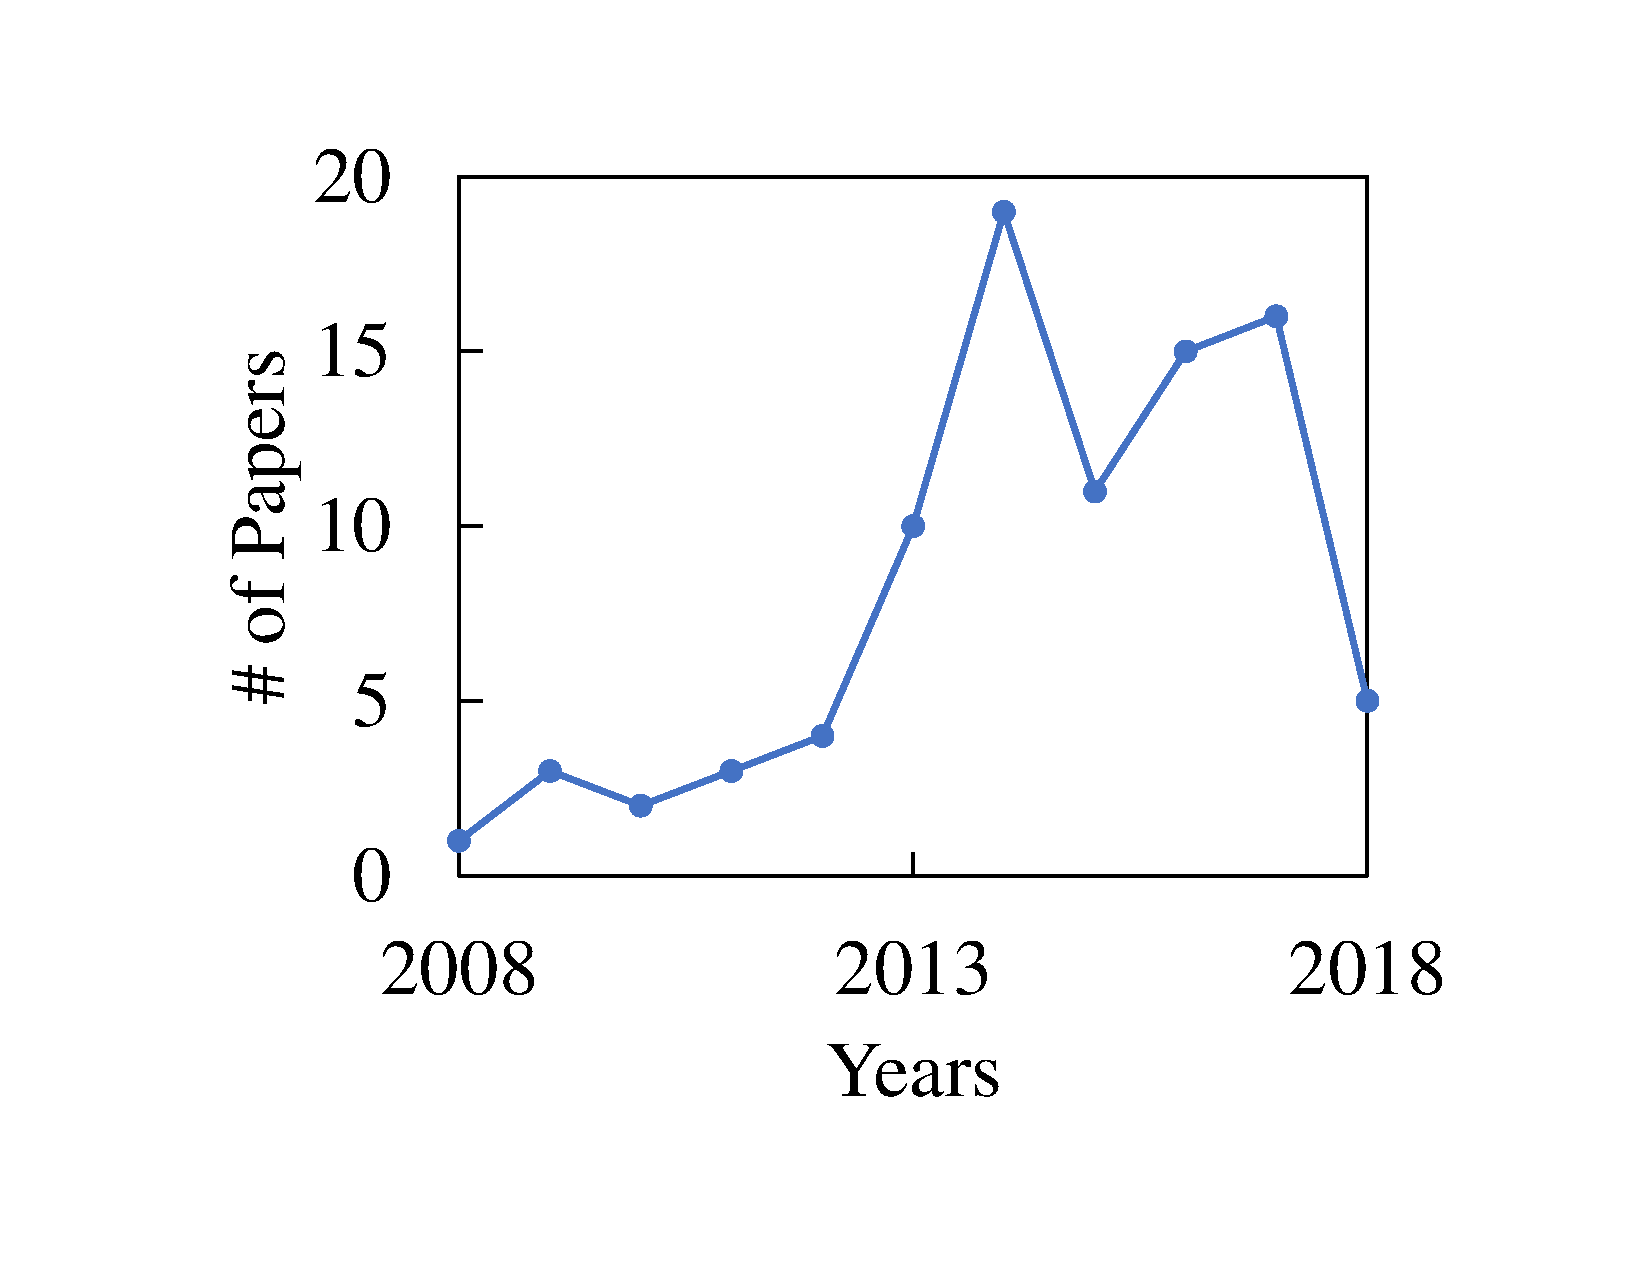
\includegraphics[width=0.7\linewidth]{figure/literature_years}
\vspace{-1.5em}
	\caption{The distribution of papers in each year}
	\vspace{-1em}
\label{fig:literature_years}
\end{figure}

The number of papers from each conference is listed in Table~\ref{tbl:literature_confs}. 
Their publication year ranges from 2008 to 2018. The detailed distributions is shown in Figure~\ref{fig:literature_years}.

c. Topic distribution 

The papers cover a large range of topics. 
Many of them are related to the detection or techniques of malwares, such as Android apps \cite{arp2014drebin,huangvt2016bigdata}, ransomware \cite{kharraz2016unveil} and Flash \cite{ford2009analyzing}. 
They mainly use \vt's detection results as baseline or ground truth. 
There are 89 papers use \vt\ to label or collect data set among the 101 papers. 
The rest 13 papers mention \vt\ for other purposes. 
We mainly focus on how the 89 papers use the detection result of \vt.

There several issues that researchers need to consider in using the results. 
First, researchers could collect detection results from multiple vendors. 
It is necessary to aggregate the results into one as the label of malware or benign for some works. 
We would like to know how researchers aggregate them. 
Second, the detection results could change over time and it is more reliable to collect the results from \vt\ during a period of time. 
We would also like to know the practice on collecting results from \vt\ over time. 
Thrid, vendors could have different impacts. 
It is also interesting to know whether and how researchers considered the different impacts of vendors.

%Last but not least, it is worth considering how we merge results from different vendors. 
First, we look at how researchers merge detection results. 
In most cases, researchers get results from more than 40 or 50 vendors and merge the results as one for their dataset. 
There are mainly two ways of merging: 1) considering a submission as malicious if any vendor can detect; 2) considering a ratio or a threshold for the number of vendors. 
For instance, Ford et al. \cite{ford2009analyzing} report it as malicious as long as there is a vendor reporting malicious
towards a file, while Carmony et al. use a threshold of 15 files. 
Among the 89 papers, 26 papers (29.2\%) use the first way and 46 papers  (51.7\%) use the second way. 
The rest 17 papers (19.1\%) do not mention how they merge results from different vendors.

Second, there are only 4 papers (4.5\%) consider that the detection results could change over time, and collect the results from \vt\ during a period of time. 
The length of time could vary from several days \cite{kharraz2016unveil, rajab2013camp} to months \cite{neeles, wressnegger2017looking}. 

Third, among the 89 papers, only 8 papers (9.0\%) consider that different vendors shall have different impact. 
Most of them pick out three to more than ten vendors to discuss their impact, because of their influence in industry or good performance on detection rate. 
For instance, Arp et al. \cite{arp2014drebin} inspected the output of ten vendors and list their detection rate anonymously. 
In addition, all of the papers treat the vendors equally. %Thomas et al. \cite{thomas2015ad} listed detection rate of 3 vendors. 
\subsection{Findings}
a. Do not wait until results become stable

b. Treat vendors equally

\subsection{Discussion}
What if the current usage is not correct? 
